% The Flink job as it actually runs: three chained tasks, two hash shuffles on the symbol.
% Taken from the job plan in results/scalability/*/job-c8-r1.json (Flink REST API) and TradingJob.java.
\documentclass[tikz,border=4pt]{standalone}
\usepackage[T1]{fontenc}
\usepackage{lmodern}
\usetikzlibrary{positioning,fit,arrows.meta,calc,backgrounds,shadows}
% Shared look for every diagram. \input this after \usetikzlibrary.
% Greys plus one accent, so the figures print fine in black and white.
\definecolor{accent}{HTML}{2563EB}
\definecolor{accentlight}{HTML}{DBEAFE}
\definecolor{latecol}{HTML}{B45309}
\definecolor{latelight}{HTML}{FEF3C7}
\definecolor{grey}{HTML}{6B7280}
\definecolor{greylight}{HTML}{F3F4F6}
\tikzset{
  box/.style={draw, rounded corners=2pt, align=center, minimum height=7mm, inner sep=3pt, fill=white, font=\footnotesize},
  topic/.style={box, fill=greylight, draw=grey},
  op/.style={box, draw=accent, fill=accentlight},
  ctr/.style={draw=grey, dashed, rounded corners=4pt, inner sep=3mm},
  note/.style={font=\scriptsize, text=grey, align=left},
  arr/.style={-{Latex[length=2mm]}, thick},
  shuffle/.style={arr, double, double distance=0.6pt, -{Latex[length=2.4mm]}},
  latearr/.style={arr, dashed, draw=latecol},
  lbl/.style={font=\scriptsize, fill=white, inner sep=1pt},
}

\tikzset{
  task/.style={draw=accent, thick, rounded corners=3pt, fill=accentlight, inner sep=2.5mm,
               double copy shadow={shadow xshift=1.4mm, shadow yshift=-1.4mm, draw=accent!60, fill=accentlight!60}},
  chained/.style={box, minimum width=38mm, font=\scriptsize},
}
\begin{document}
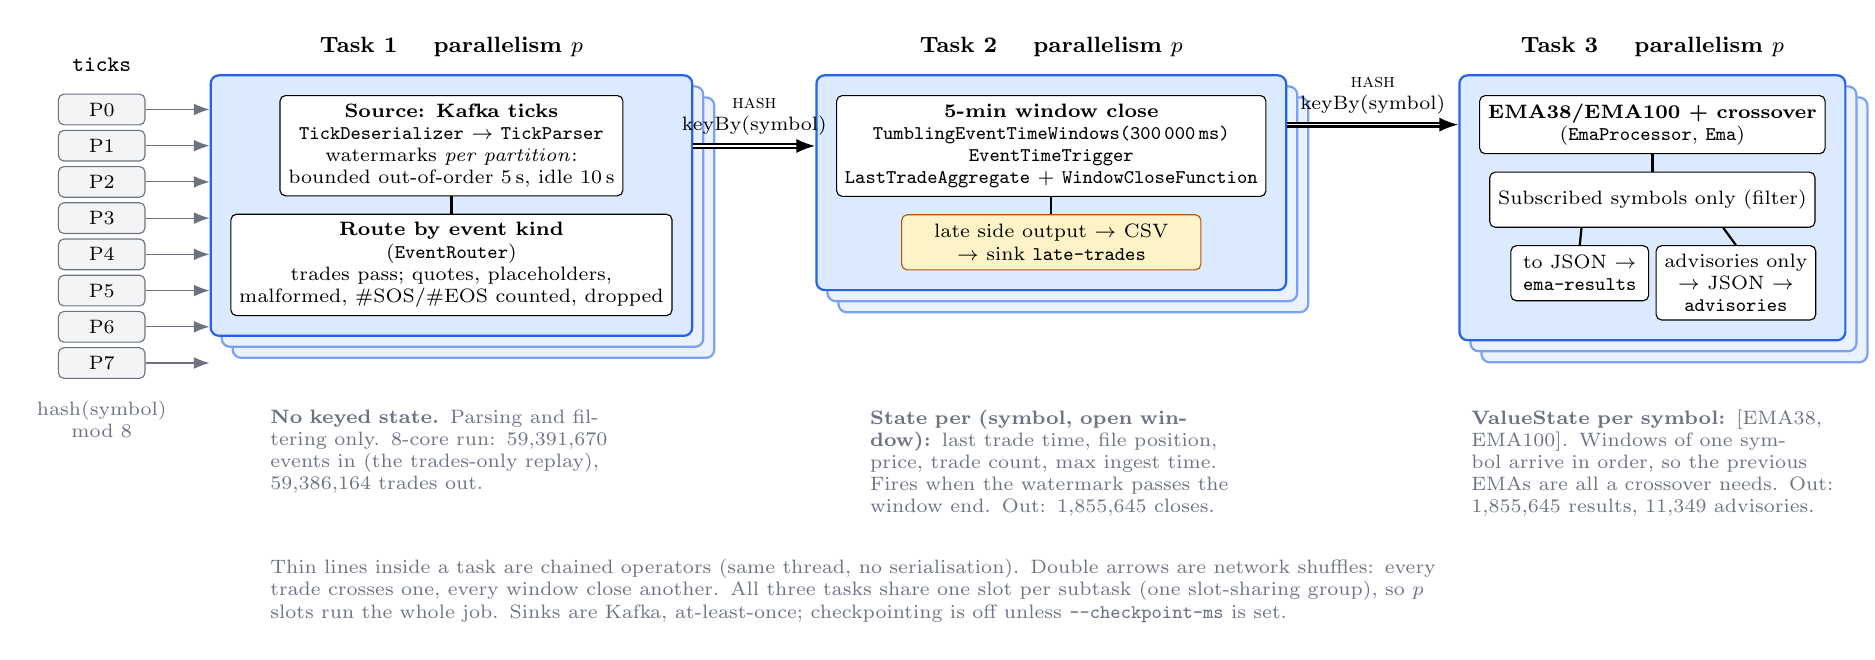
\begin{tikzpicture}[node distance=2.2mm]
  % ---------- Kafka partitions
  \foreach \i in {0,...,7} {
    \node[topic, minimum width=11mm, minimum height=3.9mm, font=\scriptsize, inner sep=1pt] (p\i) at (0,-\i*4.6mm-1mm) {P\i};
  }
  \node[font=\footnotesize\bfseries, above=1.5mm of p0] {\texttt{ticks}};
  \node[note, below=1.5mm of p7, align=center] {hash(symbol)\\mod 8};

  % ---------- Task 1
  \node[chained, right=17mm of p1] (src) {\textbf{Source: Kafka ticks}\\\texttt{TickDeserializer} $\to$ \texttt{TickParser}\\watermarks \emph{per partition}:\\bounded out-of-order 5\,s, idle 10\,s};
  \node[chained, below=of src] (route) {\textbf{Route by event kind}\\(\texttt{EventRouter})\\trades pass; quotes, placeholders,\\malformed, \#SOS/\#EOS counted, dropped};
  \begin{scope}[on background layer]
    \node[task, fit=(src)(route)] (t1) {};
  \end{scope}
  \node[font=\footnotesize\bfseries, above=1mm of t1] {Task 1 \quad parallelism $p$};

  % ---------- Task 2
  \node[chained, right=27mm of src.north east, anchor=north west] (win) {\textbf{5-min window close}\\\texttt{TumblingEventTimeWindows(300\,000\,ms)}\\\texttt{EventTimeTrigger}\\\texttt{LastTradeAggregate} + \texttt{WindowCloseFunction}};
  \node[chained, below=of win, draw=latecol, fill=latelight] (latesink) {late side output $\to$ CSV\\$\to$ sink \texttt{late-trades}};
  \begin{scope}[on background layer]
    \node[task, fit=(win)(latesink)] (t2) {};
  \end{scope}
  \node[font=\footnotesize\bfseries, above=1mm of t2] {Task 2 \quad parallelism $p$};

  % ---------- Task 3
  \node[chained, right=27mm of win.north east, anchor=north west] (ema) {\textbf{EMA38/EMA100 + crossover}\\(\texttt{EmaProcessor}, \texttt{Ema})};
  \node[chained, below=of ema] (subs) {Subscribed symbols only (filter)};
  \node[chained, below=of subs, minimum width=17.5mm, anchor=north east, xshift=-0.4mm] (j1) at (subs.south) {to JSON $\to$\\\texttt{ema-results}};
  \node[chained, minimum width=17.5mm, anchor=north west, xshift=0.4mm] (j2) at ($(subs.south)+(0,-2.2mm)$) {advisories only\\$\to$ JSON $\to$\\\texttt{advisories}};
  \begin{scope}[on background layer]
    \node[task, fit=(ema)(subs)(j1)(j2)] (t3) {};
  \end{scope}
  \node[font=\footnotesize\bfseries, above=1mm of t3] {Task 3 \quad parallelism $p$};

  % ---------- edges
  \foreach \i in {0,...,7} { \draw[arr, thin, draw=grey] (p\i.east) -- (t1.west |- p\i.east); }
  \draw[thick] (src) -- (route);
  \draw[thick] (win) -- (latesink);
  \draw[thick] (ema) -- (subs);
  \draw[thick] (subs.south) ++(-9mm,0) -- (j1.north);
  \draw[thick] (subs.south) ++(9mm,0) -- (j2.north);
  \draw[shuffle] (t1.east |- win) -- node[font=\scriptsize, above, align=center]{\textsc{hash}\\keyBy(symbol)} (t2.west |- win);
  \draw[shuffle] (t2.east |- ema) -- node[font=\scriptsize, above, align=center]{\textsc{hash}\\keyBy(symbol)} (t3.west |- ema);

  % ---------- state and counts (8-core run, 24 Nov)
  \node[note, anchor=north, text width=46mm, align=left] (n1) at ($(t1.south |- t1.south)+(0,-8mm)$) {\textbf{No keyed state.} Parsing and filtering only. 8-core run: 59,391,670 events in (the trades-only replay), 59,386,164 trades out.};
  \node[note, anchor=north, text width=46mm, align=left] (n2) at ($(t2.south |- t1.south)+(0,-8mm)$) {\textbf{State per (symbol, open window):} last trade time, file position, price, trade count, max ingest time. Fires when the watermark passes the window end. Out: 1,855,645 closes.};
  \node[note, anchor=north, text width=46mm, align=left] (n3) at ($(t3.south |- t1.south)+(0,-8mm)$) {\textbf{ValueState per symbol:} [EMA38, EMA100]. Windows of one symbol arrive in order, so the previous EMAs are all a crossover needs. Out: 1,855,645 results, 11,349 advisories.};
  \node[note, anchor=north west, text width=150mm] at ($(n1.north west)+(0,-19mm)$) {Thin lines inside a task are chained operators (same thread, no serialisation). Double arrows are network shuffles: every trade crosses one, every window close another. All three tasks share one slot per subtask (one slot-sharing group), so $p$ slots run the whole job. Sinks are Kafka, at-least-once; checkpointing is off unless \texttt{-{}-checkpoint-ms} is set.};
\end{tikzpicture}
\end{document}
